\documentclass[11pt, oneside]{article} 
\usepackage{geometry}
\geometry{letterpaper} 
\usepackage{graphicx}
	
\usepackage{amssymb}
\usepackage{amsmath}
\usepackage{parskip}
\usepackage{color}
\usepackage{hyperref}

\graphicspath{{figures/}{/Users/telliott/Github-Math/figures/}}
% \begin{center} \includegraphics [scale=0.4] {gauss3.png} \end{center}

\title{Archimedes' Quadrature Plus}
\date{}

\begin{document}
\maketitle
\Large

%[my-super-duper-separator]

Quadrature refers to the measurement of area, in particular to a method that can find the area of a plane figure.  Consider the parabola $y = x^2$ with its vertex at the origin.  
\begin{center} \includegraphics [scale=0.4] {qq1.png} \end{center}
For simplicity we will not worry about the shape factor $a$.  Pick any two points on the parabola $Q$ and $P$, with $x$-coordinates $u$ and $v$.  The $y$-coordinates of $Q$ and $P$ are $u^2$ and $v^2$.

Then find the point that lies halfway in between $(v,0)$ and $(u,0)$ and draw the vertical line $RT$ through it.  The x-coordinate of the halfway point is the average of $u$ and $v$, $(u+v)/2$.

$RT$ produces two smaller triangles of \emph{equal area}, since they have the common base $RT$ and equal height.  That height is half the horizontal distance between $P$ and $Q$
\[ h = \frac{u-v}{2} \]

It is a moderate challenge to find the length of $RT$.  The $x$-coordinates of the points $R,T$ and the intersection of $RT$ with the $x$-axis are all the same:  $(u + v)/2$.  Since $T$ is also on the curve its $y$-coordinate is the square of the $x$-coordinate $[(u + v)/2]^2 = (u+v)^2/4$ 

The $y$-coordinate of $R$ is the average of those for $P$ and $Q$ or $(u^2 + v^2)/2$. 

Finally, the length of $RT$ is difference of those two $y$-coordinates:
\[ b = \frac{u^2 + v^2}{2} - \frac{(u + v)^2}{4} \]
\begin{center} \includegraphics [scale=0.4] {qq1.png} \end{center}

Simplify this expression:
\[ 4b = 2u^2 + 2v^2 - (u^2 + 2uv + v^2) \]
\[ = u^2 - 2uv + v^2 = (u - v)^2 \]
The area of each small triangle is $hb/2$ so the area of $\triangle PQT$ is twice that:
\[ A = hb = \frac{u-v}{2} \cdot \frac{(u - v)^2}{4} \]
\[ = \frac{(u - v)^3}{8}  \]
That's a pleasingly simple result.

We ask, what would happen if we repeat the process?  Let $w$ be the $x$-coordinate of the original bisector.  Subdivide each of $PT$ and $TQ$.  Then the new distance is $u - w = (u - v)/2$.
\[ A' \stackrel{?}{=} \frac{1}{8} (\frac{u-v}{2})^3 \]

This is not quite right.  The reason is that we have here the area for the two new triangles between, say, $T$ and $Q$.  But there are also two new triangles between $P$ and $T$.  So altogether
\[ A' = 2 \cdot \frac{1}{8} (\frac{u-v}{2})^3 \]
\[ A' = \frac{1}{4} \cdot \frac{1}{8} (u - v)^3 = \frac{1}{4} A \]
Another round would yield
\[ A'' = \frac{1}{4} A' = \frac{1}{16} A \]

Thanks to a method developed by Eudoxus, we imagine that we can carry out this until the area just above the curve is \emph{exhausted}:

\[ \Delta A = A' + A'' + A''' + \dots \]
\[ = \ [ \ \frac{1}{4} + \frac{1}{16} + \dots \ ] \ A \]
\[ = \frac{1}{4} \ [ \ 1 +  \frac{1}{4} + \frac{1}{16} + \dots \ ]  \]
What lies within the brackets is a geometric series with $r = 1/4$ and (since $|r|<1$) its sum exists and is equal to
\[ \frac{1}{1 - r} = \frac{1}{3/4} = \frac{4}{3} \]
\begin{center} \includegraphics [scale=0.4] {para_series_sum.png} \end{center}
so 
\[ \Delta A = \frac{1}{4} \cdot \frac{4}{3} = \frac{1}{3} \]
\[ \frac{A + \Delta A}{A} = \frac{4}{3} \]

The total area between the curve and the secant $PQ$ is equal to $4/3$ times the area of $\triangle PTQ$.

\subsection*{checking our work}
We check this with a combination of simple calculus and not-so-simple algebra.  The area below the curve is the integral:
\[ \int_v^u x^2 \ dx = \frac{1}{3} (u^3 - v^3) \]
It will help that there is a factor of $u - v$ in the above equation:
\[ A_{\text{integral}} =  \frac{1}{3} (u - v)(u^2 + uv + v^2) \]

We said that $\triangle PTQ$ has area 
\[ \frac{1}{8} (u- v)^3 \]
\begin{center} \includegraphics [scale=0.4] {qq1.png} \end{center}

The quadrilateral formed by $PQ$, the verticals, and the $x$-axis has for its average height the $y$-value of the point $R$:
\[ h = \frac{u^2 + v^2}{2} \]
and width $u - v$ so its area is
\[ A_{\text{box}} = (u-v) \cdot \frac{u^2 + v^2}{2} \]

The areas are
\[ A_{\text{box}} = A_{\text{integral}} + \frac{4}{3} A_{\triangle} \]

We factor $u-v$ from each term before re-writing the last equation as
\[ \frac{u^2 + v^2}{2}  = \frac{1}{3} (u^2 + uv + v^2) + \frac{4}{3} \cdot  \frac{1}{8} \cdot (u-v)^2 \]
Surveying the right-hand side, clearly we have a factor of $1/3$, and that has me a little concerned as there certainly is not one on the left.

\[ = \frac{1}{3} (u^2 + uv + v^2 + \frac{(u-v)^2}{2}) \]
We expand that second term as $(u^2 - 2uv + v^2)/2$, which gives not only a cancelation but also factors of $3/2$:
\[ = \frac{1}{3} \cdot \frac{3}{2}(u^2 + v^2) = \frac{u^2 + v^2}{2} \]
And that's a relief.  $\checkmark$

\subsection*{halfway point}
The slope of the tangent to the curve at point $T$ is twice the $x$-coordinate of $T$.  That's just $2 \cdot (u + v)/2 = u + v$.

(We'll show several ways of finding the slope at any point, below.  The result here is simpler because the shape factor $a = 1$ and also the vertex is at the origin so there is no term like $bx$).  The slope of the secant $PQ$ obtained from analytic geometry is exactly the same:
\[ \frac{\Delta y}{\Delta x} = \frac{u^2 - v^2}{u - v} = u + v \]

\subsection*{any point}
Let the parabola be $y=x^2$ with points $P=(v,v^2)$ and $Q=(u,u^2)$.  The secant $PQ$ has equation $y = (u+v)x - uv$ (check both points).  The tangent $QM$ has equation $y = 2ux - u^2$ (ditto).

Let $w$ lie somewhere between $v$ and $u$, and then $T_y = w^2$.  We can get $R$ and $M$ from the equations above as $R_y = (u+v)w - uv$ and $M_y = 2uw - u^2$.
\begin{center} 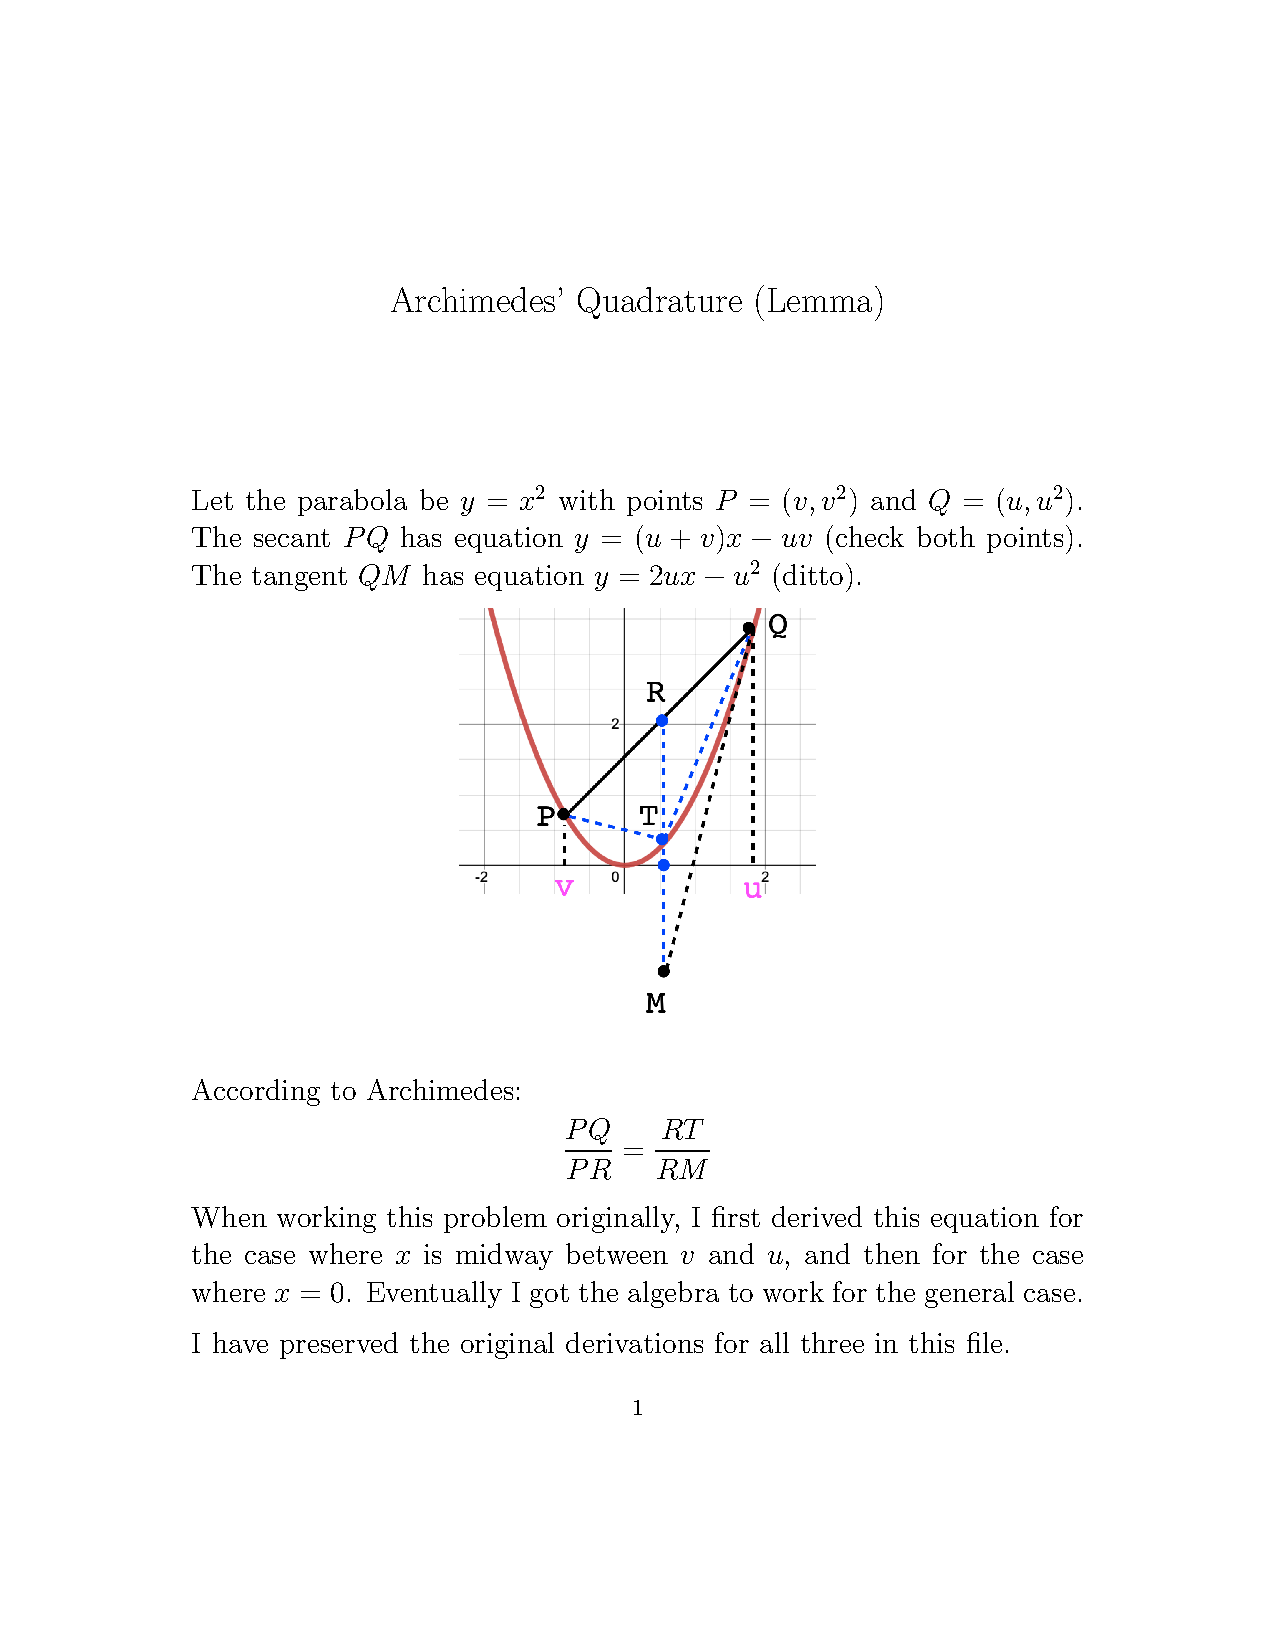
\includegraphics [scale=0.4] {qq3.png} \end{center}

The first ratio is
\[ \frac{PR}{PQ} = \frac{w-v}{u-v} \]
by similar triangles (bases and hypotenuses in same proportion;  more below *).

Then the other ratio that we want to match it is $RT/RM$.
\[ |RT| = R_y - T_y = (u+v)w - uv - w^2 \]
\[ |RM| = R_y - M_y = (u+v)w - uv - 2uw + u^2 \]
\[ = vw - uv - uw + u^2 \]
We can be guided by the first ratio.  We want $(u-v)$ on the bottom.
\[ |RM| = u(u-v) + w(v - u) = (u-v)(u-w) \]
So then let's try to find $(u-w)$ on top to get a cancelation:
\[ |RT| =  (u+v)w - uv - w^2 \]
\[ = uw - uv + wv - w^2 \]
\[ = u(w - v) + w(v-w) = (u-w)(w-v) \]
Thus
\[ \frac{RT}{RM} = \frac{(u-w)(w-v)}{(u-v)(u-w)} = \frac{w-v}{u-v} = \frac{PR}{QR} \]
$\square$

* \emph{Proof} (additional).

The secant has equation $y = kx + y_0$ where $k = (u+v)$.  So $|RP|^2$
\[ = \Delta y^2 + \Delta x^2 = \ [ \ kw - y_0 - (k v - y_0) \ ]^2 + (w - v)^2 \]
\[ (k^2 + 1)(w - v)^2 \]
$|PQ|^2$ is exactly the same, with $u$ substituted for $w$.  So in the ratio of the square roots we have just $(w-v)/(u-v)$.

\subsection*{parallel lines}
In \emph{Infinite Powers}, Strogatz describes this problem (the original one we started with) from the reverse direction.  He says that Archimedes starts with the secant and then moves that line parallel to find where it just touches the curve.

We can do that algebraically.  The equation of the secant is
\[ y = (u+v)x - uv \]
So if a point is on a line with the same slope and is also on the curve $y = x^2$:
\[ x^2 = (u+v)x - uv \]
\[ x^2 - (u+v)x + uv = 0 \]
This is a quadratic in $x$ which has a single solution when
\[ x = \frac{u+v}{2} \]
$x$ lies halfway between $u$ and $v$, as we said.

\subsection*{factor of $a$}
A factor of $a$ in the equation $y = ax^2$ stretches all $y$-values and all the areas in the $y$-direction.  The simplest way to deal with this is to do a variable substitution $y/a = u$ and then follow what we did here.

In interpreting the areas, every area will have a factor of $a$ to add back, from the stretching, and those will cancel.  We leave that as an exercise.

\subsection*{slope of the tangent}
If you've not seen calculus, you might ask why it is that if we pick two points and find the third point whose $x$ is midway, that the slope of the secant through the two points is equal to the slope of the curve at $x$.  

A French mathematician named Roberval had a beautiful answer for that.
\begin{center} \includegraphics [scale=0.4] {para20.png} \end{center}

The geometric definition of the parabola is to draw a line called the directrix and also pick a point $F$, the focus.  Then every point on the parabola $P$ has the same distance to $F$ as vertically down to $D$ on the directrix.  

We think about a particle moving along the curve.  Since the direction of ``motion'' must keep these distances exactly the same, it follows that the tangent bisects $\angle FPD$ and then $\triangle FPI \cong \triangle DPI$.  So $FPDI$ is a parallelogram.

As a result the slope of the tangent line $PI$ is $ax^2$ divided by $x/2$ which is $2ax$.

A second approach comes from calculus.  Literally the first thing we do there is to find the slope of the secant for two nearby points (separated by $\Delta x$), that satisfy a quadratic equation $y = x^2$.
\[ f'(x) = \frac{(x+\Delta x)^2 - x^2}{\Delta x} \]
\[ = \frac{2x \Delta x + (\Delta x)^2}{\Delta x} \]
\[ = 2x + \Delta x \]

The magic is that we can let $\Delta x$ ``tend'' to zero (despite having it in the denominator the moment before), and then this becomes the slope of the tangent line, which is $2x$.

A third approach is to write the equation for a line that intersects a parabola.
\[  y = kx + y_0 \]
\[ y = x^2  \]
So
\[ x^2 - kx - y_0 = 0 \]
The roots are
\[ x = \frac{k \ \pm \sqrt{k^2 - 4y_0}}{2} \]

The case of one solution is the tangent line, and that happens when the discriminant is zero.
\[ x = \frac{k}{2} \]
\[ k = 2x \]
This also constrains $y_0$ but we prefer to find it in the usual way.

\subsection*{focus}
One last thing is to talk briefly about the focus, which is the point $F = (0,f)$ with the property that for every $(x,y)$ on the parabola the distance to the focus
\[ PF = \sqrt{(x^2-f)^2 - x^2} \]
is equal to the distance to the line called the directrix $y = -f$:
\[ PD = x^2 + f \]
Thus
\[ (x^2 + f)^2 = (x^2-f)^2 - x^2 \]
\[ 2x^2f = -2x^2f - x^2 \]
\[ 4f = 1 \]
Here we just have $f = 1/4$.  The focus $F$ is the point $(0,1/4)$.  (Note $f$ does depend on the shape factor $a$.  The equation is $4af = 1$).

If we pick any points $P = (v,v^2)$ and $Q=(u,u^2)$, the line between them has slope 
\[ \frac{u^2 - v^2}{u - v} = u + v \]
and equation
\[ y = (u + v)x = uv \]
If this line also goes through $F$, then $y_0 = uv = f = -1/4$.  Multiply the slopes of the tangent lines
\[ 2u \cdot 2v = 4uv = -1 \]
We conclude that if the line connecting $P$ and $Q$ goes through the focus $F$, then the tangents through those points are perpendicular.

Here's a geometric proof from Kline.
\begin{center} \includegraphics [scale=0.35] {Kline_4_23_b.png} \end{center}

This relies on the fact that the line from the focus to any point on the parabola forms the same angle with the tangent as does the vertical.  This is the the so-called ``headlight'' property of the parabola.

Alternatively, you can accept the algebraic proof and use this as a proof of the headlight property.

\end{document}